\documentclass[17pt]{beamer} %Makes presentation
%\documentclass[handout]{beamer} %Makes Handouts
\usetheme{Singapore} %Gray with fade at top
\useoutertheme[subsection=false]{miniframes} %Supppress subsection in header
\useinnertheme{rectangles} %Itemize/Enumerate boxes
\usecolortheme{seagull} %Color theme
\usecolortheme{rose} %Inner color theme

\definecolor{light-gray}{gray}{0.75}
\definecolor{dark-gray}{gray}{0.55}
\setbeamercolor{item}{fg=light-gray}
\setbeamercolor{enumerate item}{fg=dark-gray}

\setbeamertemplate{navigation symbols}{}
%\setbeamertemplate{mini frames}[default]
%\setbeamercovered{dynamics}
\setbeamerfont*{title}{size=\Large,series=\bfseries}
\setbeamerfont{footnote}{size=\tiny}

%\setbeameroption{notes on second screen} %Dual-Screen Notes
%\setbeameroption{show only notes} %Notes Output

\setbeamertemplate{frametitle}{\vspace{.5em}\bfseries\insertframetitle}
\newcommand{\heading}[1]{\noindent \textbf{#1}\\ \vspace{1em}}

\usepackage{bbding,color,multirow,times,ccaption,tabularx,graphicx,verbatim,booktabs}
\usepackage{colortbl} %Table overlays
\usepackage[english]{babel}
%\usepackage[latin1]{inputenc}
%\usepackage[T1]{fontenc}
\usepackage{lmodern}

%\author[]{Thomas J. Leeper}
\institute[]{
  \inst{}%
  Department of Government\\London School of Economics and Political Science
}

\usepackage{tikz}
\usetikzlibrary{shapes,arrows,positioning}

\title{Concepts\\{\small ``I'll know it when I see it''}}

% Before we can study something we need to know what that ``something'' is. This is concept definition. How do we define concepts and how do we separate different concepts from one another?

\date[]{}

\begin{document}

\frame{\titlepage}

\frame{\tableofcontents}

\section{Quick Review}

\frame{\tableofcontents}
\frame{\tableofcontents[currentsection]}


\frame{
\frametitle{Fundamental problem of causal inference}

\Large We can only observe any given case in one reality! % example of taking cold medication

}


\frame{
\frametitle{In Political Science}

\begin{itemize}\itemsep0.5em
\item Causal inference is about searching for appropriate counterfactuals

\item \textit{Causal effect}: Difference in an outcome variable between two counterfactuals

\item \textit{Causal inference}: A belief that an event or variable exerts a causal effect on an outcome
\end{itemize}

}


\section{Concepts}
\frame{\tableofcontents[currentsection]}

\frame{
\frametitle{Concepts}

\begin{itemize}
\item Definition: The words and ideas that we use to describe the world

\vspace{1em}
\item<2-> Why do we care?
	\begin{itemize}\itemsep0.5em
	\item<3-> We cannot theorize or study a phenomenon until we know what it is
	\item<4-> Problem Set 1 is due on October 27.
	\end{itemize}

\end{itemize}
}

% we can look to literature or we can develop our own concepts, but as we'll talk about in a few minutes we don't want to create new concepts unless they are useful and meaningful


\frame{
\frametitle{Quick Brainstorm}

\vskip20pt

What are some important political science concepts?
}


\begin{frame}[fragile]
\frametitle{{\large Ogden \& Richard's Triangle\footnote{Richards, I.A., and Ogden, C.K. 1923 \textit{The Meaning of Meaning}.}}}

\begin{tikzpicture}
\node[align=center, text width=3.5cm] at (0,0) (label) {Label};
\node[align=center, text width=3.5cm] at (3,3) (meaning) {Meaning};
\node[align=center, text width=3.5cm] at (6,0) (cases) {Cases};

\draw[<->,very thick] (label) to (meaning);
\draw[<->,very thick] (cases) to (meaning);

\end{tikzpicture}
% meaning (set of ideas we associate with a concept; the essential constitutive elements)
% label (word used to designate a concept)
% cases (entities that are instances or cases of a concept)

\end{frame}


% distinguish concept definition from causal theorizing



\frame{

Concepts are useful because they distinguish things from other things.

\vspace{1em}

In particular, they:

\begin{itemize}
\item Resolve ambiguity
% label connected to multiple meanings
% meaning connected to multiple labels

\item Avoid vagueness % lack of a good definition
\end{itemize}

}

% For example, if we want to build an understanding of the concept ``democracy'' (such as its effects on economic outcomes, or the processes that cause democracies to form) then we need to be clear about what we mean by democracy. We need to distinguish it from other concepts that might be related but that are different (autocracy, oligarchy, anarchy, state, nation-state, liberal society, etc.).

\frame{
\frametitle{{\normalsize Approaches to Concept Definition}}

\begin{enumerate}
\item Classical Approach
\item Family Resemblence
\end{enumerate}

\vspace{1em}

\begin{itemize}
\item Gerring's 7 criteria\footnote{Gerring also offers ``minimal,'' ``maximal,'' and ``cumulative'' formulations as ways to develop concepts}
\end{itemize}
}

% Gerring distinguishes between minimal (classical approach); maximal (ideal types; Think Dahl and democracy as an ideal type); cumulative (more or less of a concept)
% the last of these will be particularly helpful when we start thinking about operationalization or measurement next week


\section[Classical Approach]{Concepts: Classical Approach}
\frame{\tableofcontents[currentsection]}


\frame{
\frametitle{Classical Approach}


\begin{itemize}\itemsep0.5em
\item Specify a set of ``constitutive dimensions'' that \textit{are} the concept
	\begin{itemize}
	\item Fundamental characteristics of the concept
	\item Not causes or effects
	\item Not measures of the concept
	\end{itemize}
\item<2-> Dimensions are \textit{necessary and jointly sufficient}

\end{itemize}
}


\frame{
\frametitle{Boolean Logic}

\begin{itemize}\itemsep0.5em
\item \textbf{AND}: necessary
	\begin{itemize}
	\item Implies attributes required to be a case of the concept
	\end{itemize}
\item \textbf{OR}: sufficient
	\begin{itemize}
	\item Implies multiple ways to be a case of the concept
	\end{itemize}
\end{itemize}

Attributes may be \textit{individually} or \textit{jointly} necessary and/or sufficient
}



\frame{
\frametitle{{\large Dahl's Definition of Democracy}}

\begin{itemize}
\item Two dimensions
	\begin{itemize}
	\item<2-> Liberalization (Public contestation)
	\item<2-> Inclusiveness (Participation)
	\end{itemize}
\item Both necessary and jointly sufficient
\item<3-> Without liberalization: ``inclusive hegemony''
\item<4-> Without inclusiveness: ``competitive oligarchy''
\end{itemize}

}

% discuss joint necessity and sufficiency


\frame{
\frametitle{Minimal and Maximal}

\begin{itemize}\itemsep0.5em
\item Gerring uses three types of concept definitions:
	\begin{itemize}
	\item Minimal
	\item Maximal
	\item Cumulative
	\end{itemize}
\item All three of these are within the classical approach
	\begin{itemize}
	\item All focus attribute \textit{necessity}
	\end{itemize}
\end{itemize}
}


\frame{\huge\vskip20pt\textbf{Questions?}}

\frame[label=chairexample]{

\title{Example}

Define the concept of ``\hyperlink{chairs}{chair}''

\begin{center}

\includegraphics[height=0.7\textheight]{images/chair}
\end{center}

{\tiny \href{https://commons.wikimedia.org/wiki/File:Chair_5709.jpg}{Image Source: Wikimedia} by \href{https://commons.wikimedia.org/wiki/User:Dori}{User:Dori}}
}


\section[Family Resemblence]{Concepts: Family Resemblence}
\frame{\tableofcontents[currentsection]}

\frame{
\frametitle{Family Resemblence}

\begin{itemize}
\item Classical approach focuses on \textit{necessary} elements
\item Some concepts have no necessary elements but are still meaningful % Game
\item<2-> We might also think about elements that are \textit{sufficient} to establish membership
\end{itemize}
}


\begin{frame}[label=game, fragile]

\frametitle{Example: Define ``game''}

\vspace{-2.2em}

\begin{center}
\resizebox{\textwidth}{0.75\textheight}{%
\begin{tikzpicture}
  \node (img1) {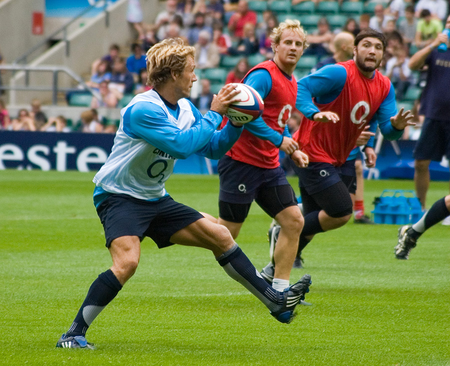
\includegraphics[height=3cm]{images/rugby}};
  \node (img2) [below right=-1cm and -1.5cm of img1] {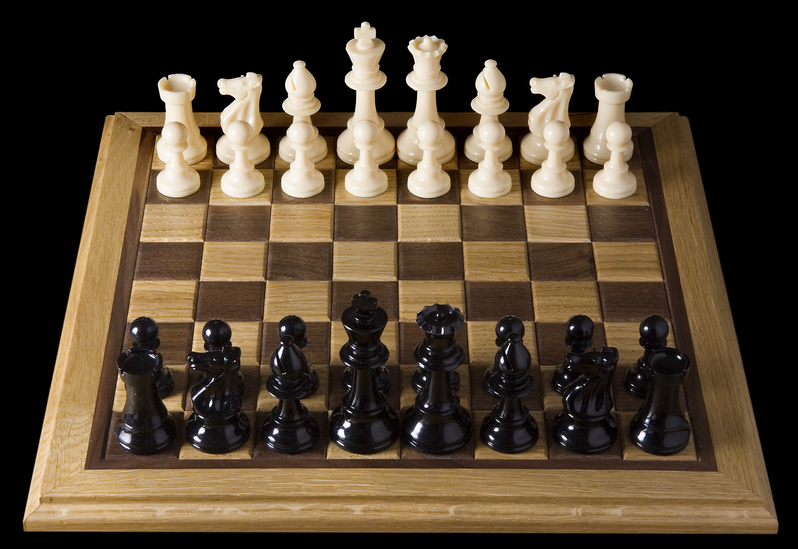
\includegraphics[height=3cm]{images/chess}};
  \node (img3) [below=-0.5cm of img1] {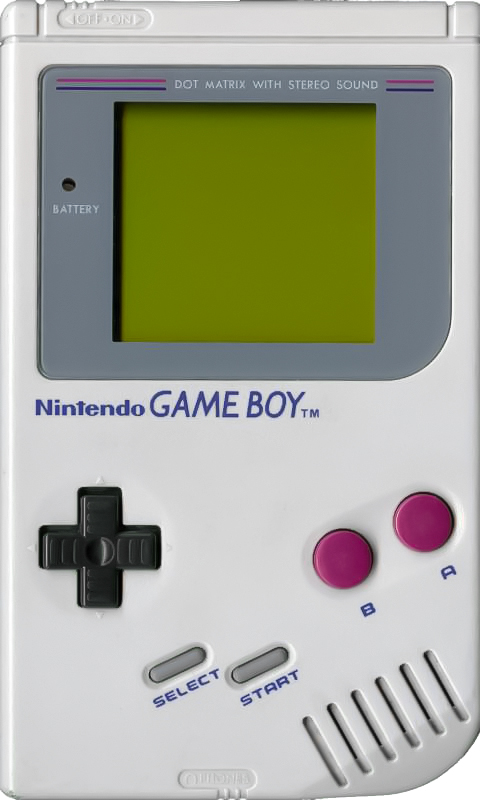
\includegraphics[height=3cm]{images/gameboy}};
  \node (img4) [above right=-2.5cm and -0.25cm of img1]  {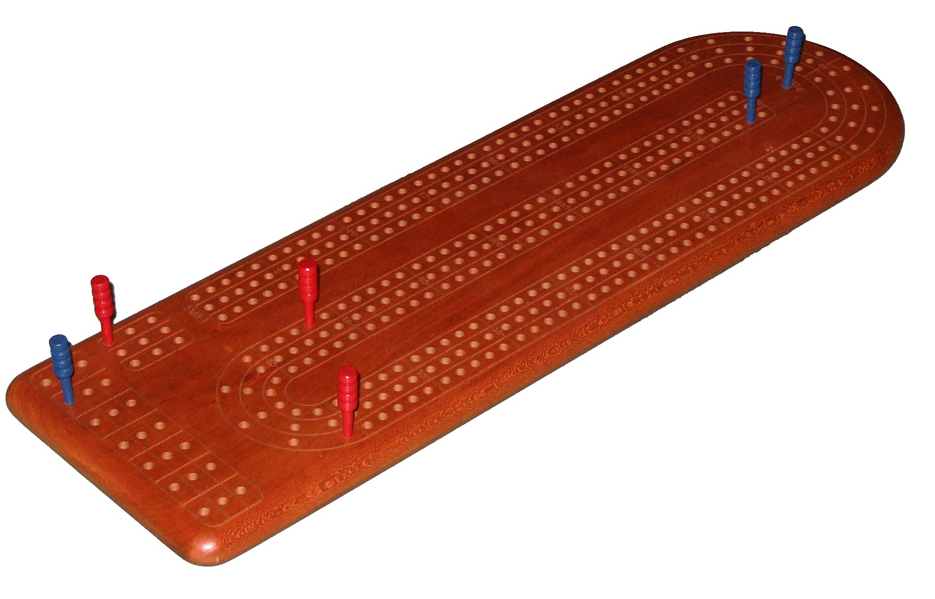
\includegraphics[height=3cm]{images/cribbage}};
  \node (img5) [below right=0.5cm and -2cm of img4]  {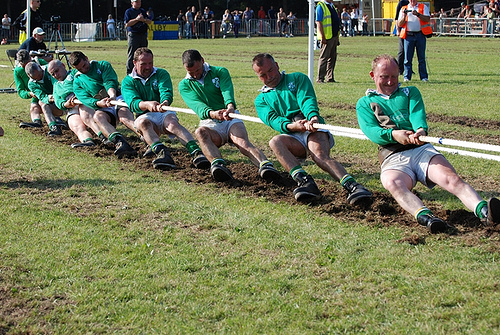
\includegraphics[height=3cm]{images/tugofwar}};
  \node (img6) [above right=-1cm and 0.5cm of img2]  {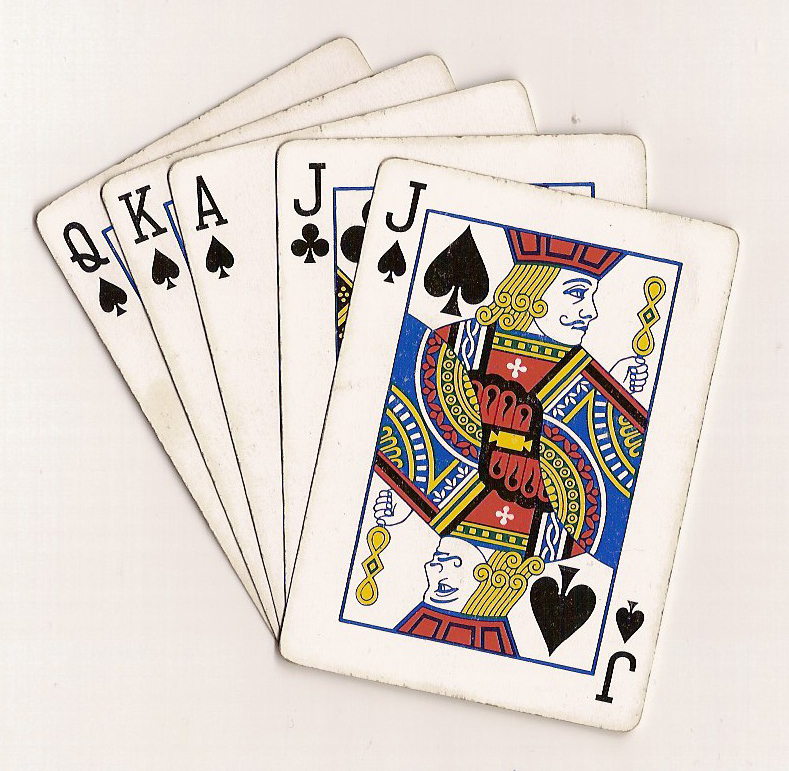
\includegraphics[height=3cm]{images/cards}};
\end{tikzpicture}
}
\end{center}

\vspace{-1em}

\hyperlink{gamesources}{\beamergotobutton{Image Sources}}

\end{frame}


\frame{
\frametitle{Complex Boolean Logic}

\small

\begin{itemize}\itemsep0.5em

\item Jointly necessary and sufficient:\\
\hspace{1em} {\footnotesize $\text{Rule of Law} \land \text{Equality}$}

\item Jointly necessary w/ insufficient attributes\\
\hspace{1em} {\footnotesize $\text{Rule of Law} \land (\text{Equality} \lor \text{Elections}) $}

\item Simple family resemblance logic:\\
\hspace{1em} {\footnotesize $(\text{Equality} \lor \text{Elections})$}

\item Complex family resemblance logic:\\
\hspace{1em} {\footnotesize $(\text{Rule of Law} \land \text{Participation}) \lor (\text{Equality} \land \text{Elections}) $}

\end{itemize}

}



\begin{frame}[fragile]

\frametitle{Trade-offs}

\vspace{-2em}

\begin{center}
\begin{tikzpicture}
	% x-axis
    \draw[->] (0,0) node[below] (origin) {} -- (5,0) node[right] (xaxis) {};
    \node[below] at (2.5,-0.75) {\small Intension (More attributes)};
	\node[below] at (0.5,0) {\footnotesize Low};
	\node[below] at (5,0) {\footnotesize High};
	
	% y-axis
    \draw[->] (origin) -- (0,5) node[left] (yaxis) {};
	\node[left, text width=5cm, align=center] at (0,2.5) {\small Extension\\(More cases)};
	\node[left] at (0,0.5) {\footnotesize Low};
	\node[left] at (0,5) {\footnotesize High};

    \draw[<->, solid] (0.5,4.5) -- (4.5,0.5);
    \node[above, rotate=45] at (4,4) {\tiny Sufficient};
    
    \draw[<->, dashed] (0.5,0.5) -- (4.5,4.5);
    \node[rotate=-45] at (4,1.25) {\tiny Necessary};

\end{tikzpicture}
\end{center}
\end{frame}

% Need to balance specificity against abstraction/generality
% In classical approach, intension and extension are inversely related (Gerring Fig. 5.1)
% In family resemblence approach, intension and extension are positively related
% If we increase necessary attributes, we have fewer cases of that concept and it is more specific
% If we increase sufficient attributes, we have more cases of that concept and it is more general



\frame{\huge\vskip20pt\textbf{Questions?}}


\section{Gerring's Criteria}
\frame{\tableofcontents[currentsection]}

\frame{
\frametitle{Gerring's Criteria}

\begin{enumerate}
\item Resonance
\item Domain/scope % ladder of generality
\item Consistency
\item Fecundity
\item Differentiation
\item Causal utility
\item Operationalization (next week)
\end{enumerate}
}

% divide these up and have someone present each one


% Resonance: Is the concept intuitive? Avoid neologism (Gerring p.118); we don't need new terms for the sake of having new terms

% Domain: The contexts in which this concept resonates and applies. Example: "vouchers". What does this mean? This has a clear meaning in the United States, in debates about education policy, but that is a narrow domain. Contrast this with democracy or terrorism, which are concepts with broad domains.

% Consistency: We can change the definition of a concept by adding, removing, or modifying attributes; Contrast with "slippage" or "stretching"

% Fecundity: Fertility or fruitfulness; Neologisms are prone to lacking fecundity

% Differentiation: How does this concept contrast or help create distinctions between existing sets of phenomena? Example: *Opinion* is a summary evaluation of a particular object; *Value* is a belief about a desired end-state of the world

% Causal Utility: Concept has to be useful for making a causal argument; this may require a concept to be more specific or have higher intensity than we would prefer because we need to *use* the concept

% Operationalization: concepts have to be measurable; we'll talk about this next week


\section*{}

\frame{

\frametitle{In Sum}

\begin{itemize}\itemsep0.5em
\item We need to know what we're talking about before we can theorize causal relationships or study something empirically
\item Concept vary in their usefulness and are contestable
\item Many ways to define and evaluate concepts
\end{itemize}

}



\appendix
\frame{}

\frame[label=gamesources]{

\tiny

\begin{itemize}
\item Rugby: flickr user Paddy-K \url{https://commons.wikimedia.org/wiki/File:Jonny_Wilkinson_2009_08_england_training_2.jpg}
\item Chess: Wikimedia user MichaelMaggs \url{https://commons.wikimedia.org/wiki/File\%3AOpening_chess_position_from_black_side.jpg}
\item Gameboy: Public domain \url{https://commons.wikimedia.org/wiki/File\%3AGameboy.jpg}
\item Cribbage: Wikimedia user Aerion \url{https://commons.wikimedia.org/wiki/File:120-hole_cribbage_board.jpg}
\item Cards: Public domain \url{https://commons.wikimedia.org/wiki/File\%3AEuchre.jpg}
\item Tug of war: Wikimedia user Johnmoore6 \url{https://en.wikipedia.org/wiki/File:Irish_600kg_euro_chap_2009.JPG}
\end{itemize}

\hyperlink{game}{\beamergotobutton{Return to Images}}

}

\frame[label=chairsources]{

\tiny

\begin{itemize}
\item images/chair: Wikimedia user Dori \url{https://commons.wikimedia.org/wiki/File:Chair_5709.jpg}
\item images/throne: Wikimedia user Badseed  \url{https://commons.wikimedia.org/wiki/File:Ottoman_throne.jpg}
\item images/beanbag: Wikimedia user Pava  \url{https://commons.wikimedia.org/wiki/File:\%22_12_-_ITALY_-_Pouf_Tuffet_Sacco_di_Zanotta_red_armchair_Triennale_Design_Museum.jpg}
\item images/kneelingchair: Wikimedia user TonyTheTiger  \url{https://commons.wikimedia.org/wiki/File:Deluxe_kneeling_chair.jpg}
\item images/bench: Wikimedia user 4028mdk09  \url{https://commons.wikimedia.org/wiki/File:Holzbank_mit_schmiedeeisener_R\%C3\%BCckenlehne.JPG}
\item images/trainseat: Wikimedia user Lover Of Romance \url{https://commons.wikimedia.org/wiki/File:Green-Car\%27s_Seat_of_JR_215.JPG}
\item images/hermanmiller: Wikimedia user Luiscarlosrubino \url{https://commons.wikimedia.org/wiki/File:Mirra_Chair_by_Studio_7.5_-_Herman_Miller.jpg}
\item images/wc: Public Domain \url{https://commons.wikimedia.org/wiki/File:Wc1.jpg}
\item images/stool: Wikimedia user Chatsam \url{https://commons.wikimedia.org/wiki/File:Pied_d\%27\%C3\%A9l\%C3\%A9phant_marche_pied.jpg}

\end{itemize}

\hyperlink{chairs}{\beamergotobutton{Return to Images}}

}

\frame[label=chairs]{


\includegraphics[width=2.25cm]{images/chair}
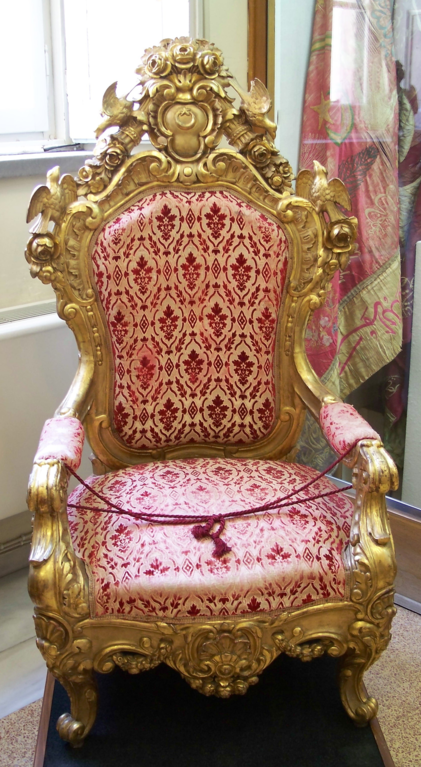
\includegraphics[width=1.75cm]{images/throne}

\includegraphics[width=2.25cm]{images/hermanmiller}

\includegraphics[width=1.75cm]{images/wc}
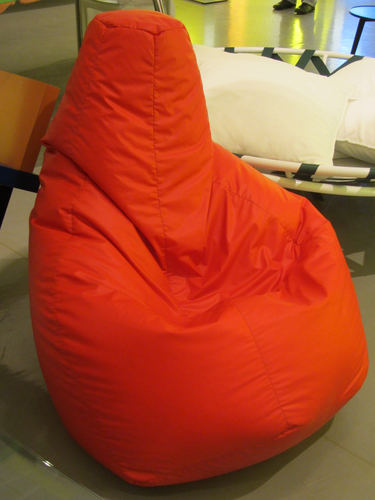
\includegraphics[width=2.7cm]{images/beanbag}

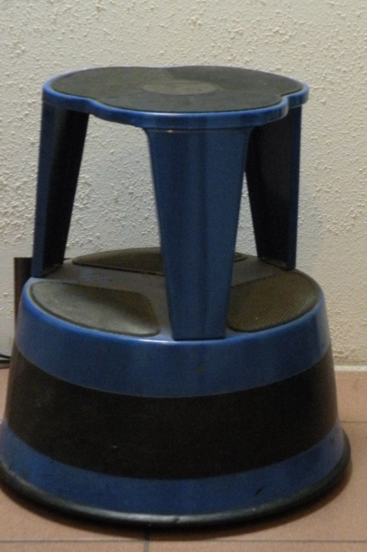
\includegraphics[width=2.5cm]{images/stool}
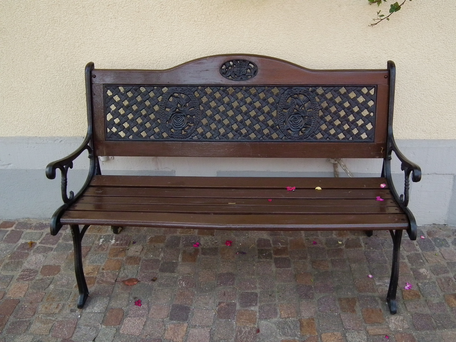
\includegraphics[width=5cm]{images/bench}
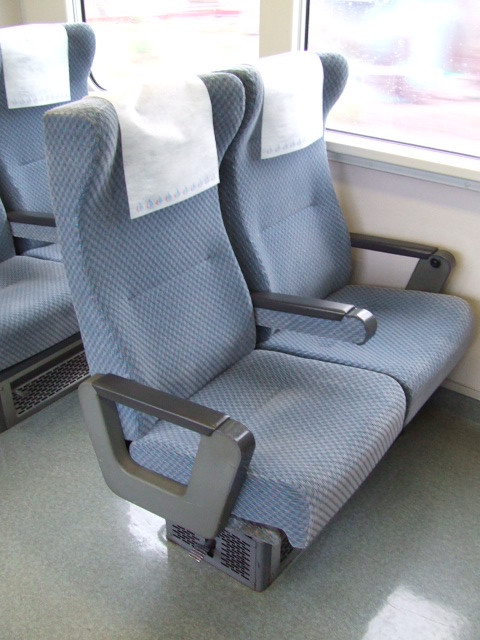
\includegraphics[width=2.8cm]{images/trainseat}

\hyperlink{chairexample}{\beamergotobutton{Return to Slides}} \hyperlink{chairsources}{\beamergotobutton{Image Sources}}

}

\end{document}
